% First draft: 1977_fujian_science_q1_fig1 (trapezoid, trisection lines).
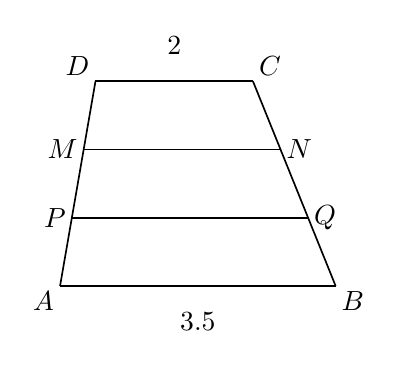
\begin{tikzpicture}[x=1cm,y=1cm,font=\normalsize,
 geometry edge/.style={solid,line width=.6pt},
 geometry mark/.style={solid,line width=.6pt},
 geometry label/.style={font=\normalsize,inner sep=2pt}]
\coordinate (D) at (0.0000,2.6000);
\coordinate (C) at (2.0000,2.6000);
\coordinate (A) at (-0.4500,0.0000);
\coordinate (B) at (3.0500,0.0000);
\coordinate (M) at (-0.1500,1.7333);
\coordinate (N) at (2.3500,1.7333);
\coordinate (P) at (-0.3000,0.8667);
\coordinate (Q) at (2.7000,0.8667);
\draw[geometry edge] (D)--(C);
\draw[geometry edge] (C)--(B);
\draw[geometry edge] (B)--(A);
\draw[geometry edge] (A)--(D);
\draw[geometry edge] (M)--(N);
\draw[geometry edge] (P)--(Q);
\node[geometry label,above left] at (D) {$D$};
\node[geometry label,above right] at (C) {$C$};
\node[geometry label,below left] at (A) {$A$};
\node[geometry label,below right] at (B) {$B$};
\node[geometry label,left] at (M) {$M$};
\node[geometry label,right] at (N) {$N$};
\node[geometry label,left] at (P) {$P$};
\node[geometry label,right] at (Q) {$Q$};
\node[font=\normalsize] at (1.0000,3.0500) {$2$};
\node[font=\normalsize] at (1.3000,-0.4500) {$3.5$};
\end{tikzpicture}
